% Created 2016-08-21 Sun 10:52
\documentclass[presentation]{beamer}
\usepackage[utf8]{inputenc}
\usepackage[T1]{fontenc}
\usepackage{fixltx2e}
\usepackage{graphicx}
\usepackage{longtable}
\usepackage{float}
\usepackage{wrapfig}
\usepackage{rotating}
\usepackage[normalem]{ulem}
\usepackage{amsmath}
\usepackage{textcomp}
\usepackage{marvosym}
\usepackage{wasysym}
\usepackage{amssymb}
\usepackage{hyperref}
\tolerance=1000
\usepackage{tabu}
\usepackage{minted}
\hypersetup{pdfauthor="Vasilij Schneidermann", pdftitle="MAL - Making a Lisp", colorlinks, linkcolor=black, urlcolor=blue}
\usetheme{Rochester}
\usecolortheme[RGB={87,83,170}]{structure}
\author{Vasilij Schneidermann}
\date{August 2016}
\title{MAL - Making a Lisp}
\hypersetup{
  pdfkeywords={},
  pdfsubject={},
  pdfcreator={Emacs 24.5.1 (Org mode 8.2.10)}}
\begin{document}

\maketitle
\begin{frame}{Outline}
\tableofcontents
\end{frame}

\AtBeginSection{\frame{\sectionpage}}

\section{Einführung}
\label{sec-1}

\begin{frame}[label=sec-1-1]{Sprecher}
\begin{itemize}
\item Vasilij Schneidermann, 24
\item Wirtschaftsinformatikstudent
\item Praktikant bei \href{https://www.bevuta.com/en/}{bevuta IT GbmH}
\item \texttt{v.schneidermann@gmail.com}
\item \url{https://github.com/wasamasa}
\item \url{http://emacshorrors.com/}
\item \url{http://emacsninja.com/}
\end{itemize}
\end{frame}

\begin{frame}[fragile,label=sec-1-2]{Motivation}
 \begin{itemize}
\item Lisp relativ einfach erlernbar
\item Feinheiten weniger
\item Quoting, Makros, Environments, \texttt{eval}, etc.
\item Besseres Verständnis durch Implementieren von Lisp!
\item \href{https://github.com/kanaka/mal}{MAL} in vieler Hinsicht ideal
\item Durch den Sprecher in Emacs Lisp und ChucK implementiert
\end{itemize}
\end{frame}

\begin{frame}[label=sec-1-3]{Was ist MAL?}
\begin{itemize}
\item Minimale, an \href{http://clojure.org/}{Clojure} angelehnte Programmiersprache
\item Lisp-Implementierung in vielen Sprachen, \href{https://en.wikipedia.org/wiki/Meta-circular_evaluator}{inklusive MAL}
\item Showcase à la \href{http://rosettacode.org/wiki/Rosetta_Code}{Rosetta Code}
\item Anleitung zum Interpreter-Bau
\item Pädagogisches Werkzeug
\item Einbettbar!
\end{itemize}
\end{frame}

\begin{frame}[label=sec-1-4]{Warum nicht Scheme?}
\begin{itemize}
\item \href{http://schemers.org/}{Scheme} ist deutlich größer
\item Herausfordernder (call/cc, hygienische Makros, RNRS)
\item Weniger Hilfestellung gegeben
\item Etwas weniger praktikabel als Clojure (weniger eingebaute Datenstrukturen)
\item Alternativ: \href{http://thinking-forth.sourceforge.net/}{Forth}, \href{http://pharo.org/}{Smalltalk}
\end{itemize}
\end{frame}

\section{MAL}
\label{sec-2}

\begin{frame}[label=sec-2-1]{Historie}
\begin{itemize}
\item Autor: Joel Martin (\href{https://github.com/kanaka}{@kanaka})
\item Inspiration durch \href{https://github.com/alandipert/gherkin}{gherkin} (Lisp in Bash 4)
\item Schrieb ein Lisp in GNU Make (MAke Lisp)
\item Abstrahierte die Gemeinsamkeiten weiterer Implementierungen
\item Umbenennung zu Make A Lisp
\end{itemize}
\end{frame}

\begin{frame}[label=sec-2-2]{Fun Facts}
\begin{itemize}
\item Lizenz: MPL 2.0
\item Contributors: 49
\item Implementierungen: 57
\item Schritte: 11
\item Unit Tests: 636
\end{itemize}
\end{frame}

\begin{frame}[fragile,label=sec-2-3]{Sprache}
 \begin{itemize}
\item Abgespecktes Clojure
\item Keine Namespaces, Concurrency, Lazy Sequences, Protokolle,
Multimethods, First-Class Interop, \ldots{}
\item \texttt{true}, \texttt{false}, \texttt{nil}, Int, String, Symbol, Keyword, List, Vector,
Hash Map, Atom
\item Unterstützt Variablen, Funktionen, Environments, Closures, TCO, IO,
\texttt{eval}, Quoting, Makros, Exceptions, Metadaten
\item 57 Subrs, 10 Special Forms, 5 in der Sprache definierte Formen
\item Hinreichend für Self-Hosting
\end{itemize}
\end{frame}

\begin{frame}[fragile,label=sec-2-4]{Code-Beispiele}
 Aus \href{https://github.com/kanaka/mal/blob/master/process/guide.md}{dem Guide} entnommen:

\begin{minted}[]{clojure}
(def! not
  (fn* [x]
    (if x false true)))

(def! load-file
  (fn* [f]
    (eval
     (read-string
      (str \"(do \" (slurp f) \")\")))))
\end{minted}
\end{frame}

\begin{frame}[fragile,label=sec-2-5]{Code-Beispiele}
 Triviales Makro:

\begin{minted}[]{clojure}
(defmacro! comment
  (fn* [& body]
    nil))
\end{minted}

Exceptions:

\begin{minted}[]{clojure}
(try* (/ 1 0) (catch* ex (prn "Prevented doom")))
;; "Prevented doom"
;; nil
\end{minted}

Einfache Rekursion:

\begin{minted}[]{clojure}
(def! fact
  (fn* [x]
    (if (<= x 1)
      x
      (* x (fact (- x 1))))))
\end{minted}
\end{frame}

\begin{frame}[fragile,label=sec-2-6]{Code-Beispiele}
 Komplexere Rekursion:

\begin{minted}[]{clojure}
(def! reverse
  (let* [reverse*
         (fn* [arg acc]
           (let* [xs (seq arg)]
             (if xs
               (reverse* (rest xs) (cons (first xs) acc))
               acc)))]
    (fn* [xs] (reverse* xs ()))))
\end{minted}
\end{frame}

\begin{frame}[label=sec-2-7]{Hilfestellung}
\begin{itemize}
\item Vorgefertige Make-Targets
\item Viele Unit Tests
\item CI
\item Guide
\item Cheatsheet
\item Überschaubare Implementierungsschritte
\item Balance zwischen Aha-Momenten und Schwierigkeit
\end{itemize}
\end{frame}

\begin{frame}[fragile,label=sec-2-8]{Community}
 \begin{itemize}
\item IRC-Channel auf Freenode, \texttt{\#mal}
\item GitHub
\end{itemize}
\end{frame}

\section{Implementierung}
\label{sec-3}

\begin{frame}[label=sec-3-1]{Auswahl einer geeigneten Implementierungssprache}
\begin{itemize}
\item Theoretisch jede Turing-vollständige Sprache denkbar
\item Abstrusere Beispiele:
\begin{itemize}
\item AWK
\item Bash
\item ChucK
\item Emacs Lisp / VimScript
\item LOGO
\item GNU Make
\item MATLAB / R
\item PL/pgSQL / PL/SQL
\item PostScript
\item Visual Basic
\item VHDL
\end{itemize}
\end{itemize}
\end{frame}

\begin{frame}[label=sec-3-2]{Auswahl einer geeigneten Implementierungssprache}
\begin{itemize}
\item Schon verwendete Sprachen im Repository
\item \url{https://lobste.rs/}
\item \url{http://www.tiobe.com/tiobe-index/}
\item \url{http://langpop.corger.nl/}
\item \url{https://en.wikipedia.org/wiki/List_of_programming_languages}
\item \url{http://rosettacode.org/wiki/Rosetta_Code}
\end{itemize}
\end{frame}

\begin{frame}[fragile,label=sec-3-3]{Wünschenswerte Features}
 \begin{itemize}
\item Sequentielle Datenstruktur (Array, Liste, Vektor)
\item Assoziative Datenstruktur (Dictionary, Hash Table/Map, Assoziatives Array)
\item Funktionsreferenzen (Funktionspointer, First-Class Functions, Delegates)
\item Exception Handling (\texttt{try}, \texttt{catch}, \texttt{throw})
\item Varargs (\texttt{apply}, Splat-Operator, \texttt{...})
\item Lexikalische Closures
\item Reguläre Ausdrücke (nötig für \texttt{READ})
\end{itemize}
\end{frame}

\begin{frame}[fragile,label=sec-3-4]{Erforderliche Features}
 \begin{itemize}
\item Zahlen(!)
\item (Erweiterbare) Objekte, Structs, Records
\item Brauchbares statisches Typsystem / dynamische Typisierung
\item IO für Konsolen-Input, -Output und Auslesen von Dateien
\item Präzise Zeitmessung (alternativ "Shelling out")
\item Laden von Code aus anderen Dateien (Module, \texttt{require}, \texttt{import})
\item Linux-Support (alternativ OS X, Windows), Aufruf aus Konsole
\end{itemize}
\end{frame}

\begin{frame}[label=sec-3-5]{Schritt 0}
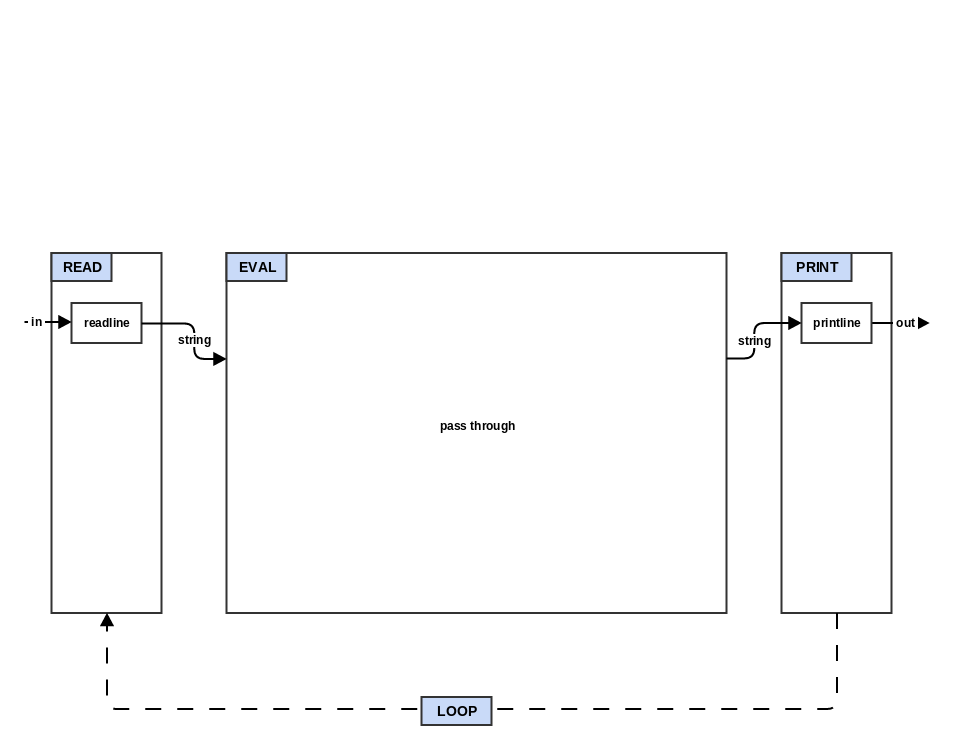
\includegraphics[width=.9\linewidth]{./images/step0_repl.png}
\end{frame}

\begin{frame}[label=sec-3-6]{Schritt 0}
\begin{itemize}
\item REPL
\item Grundlegende Konsolen-IO erforderlich
\item Einlesen von Benutzereingabe sollte abbrechbar sein
\item Falls nötig, kann zu Hacks gegriffen werden\ldots{}
\item Sanity Check des Testgerüsts
\item Optional: Readline
\end{itemize}
\end{frame}

\begin{frame}[label=sec-3-7]{Schritt 1}
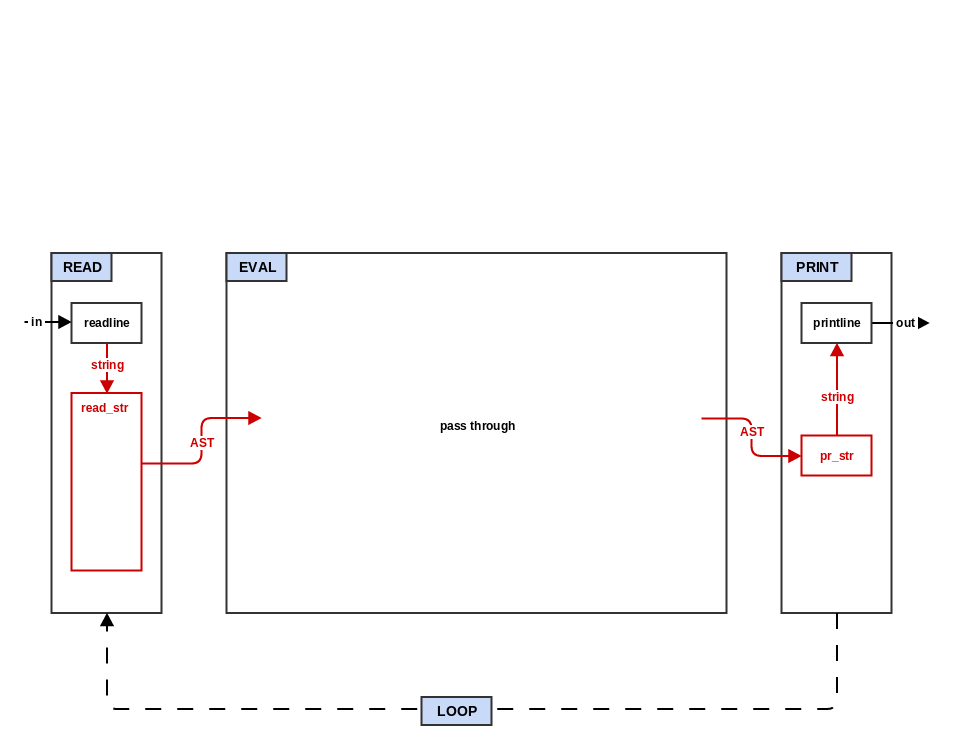
\includegraphics[width=.9\linewidth]{./images/step1_read_print.png}
\end{frame}

\begin{frame}[fragile,label=sec-3-8]{Schritt 1}
 \begin{itemize}
\item \texttt{READ}
\item Aufteilung der Eingabe in Tokens
\item \texttt{(+ 1 1)} -> \texttt{(}, \texttt{+}, \texttt{1}, \texttt{1}, \texttt{)}
\item Bevorzugt mit RE, ansonsten von Hand
\item \texttt{[\textbackslash{}s,]*(\textasciitilde{}@|[\textbackslash{}[\textbackslash{}]\{\}()'`\textasciitilde{}\textasciicircum{}@]|"(?:\textbackslash{}\textbackslash{}.|[\textasciicircum{}\textbackslash{}\textbackslash{}"])*"| ;.*|[\textasciicircum{}\textbackslash{}s\textbackslash{}[\textbackslash{}]\{\}('"`,;)]*)}
\item Reader liest eine \emph{Form} aus Tokens
\item Entweder ein Skalar oder eine Liste/Vektor/Map aus weiteren Formen
\item Minimale Fehlerbehandlung
\item Reader-Makros werden zu Objekten konvertiert
\end{itemize}
\end{frame}

\begin{frame}[fragile,label=sec-3-9]{Schritt 1}
 \begin{itemize}
\item \texttt{PRINT}
\item Wesentlich einfacher
\item Skalare werden direkt zu Strings konvertiert, komplexere Formen
rekursiv
\item Printer muss in der Lage sein besondere Zeichen "lesbar" zu drucken
(\texttt{print} vs. \texttt{prn})
\item Alle Typen müssen repräsentierbar sein
\item Korrekte Behandlung von Kommentaren und Newlines
\item Schwierigster Schritt, da Parsen, Drucken und Umsetzung des
Typsystems von MAL notwendig sind
\end{itemize}
\end{frame}

\begin{frame}[label=sec-3-10]{Schritt 2}
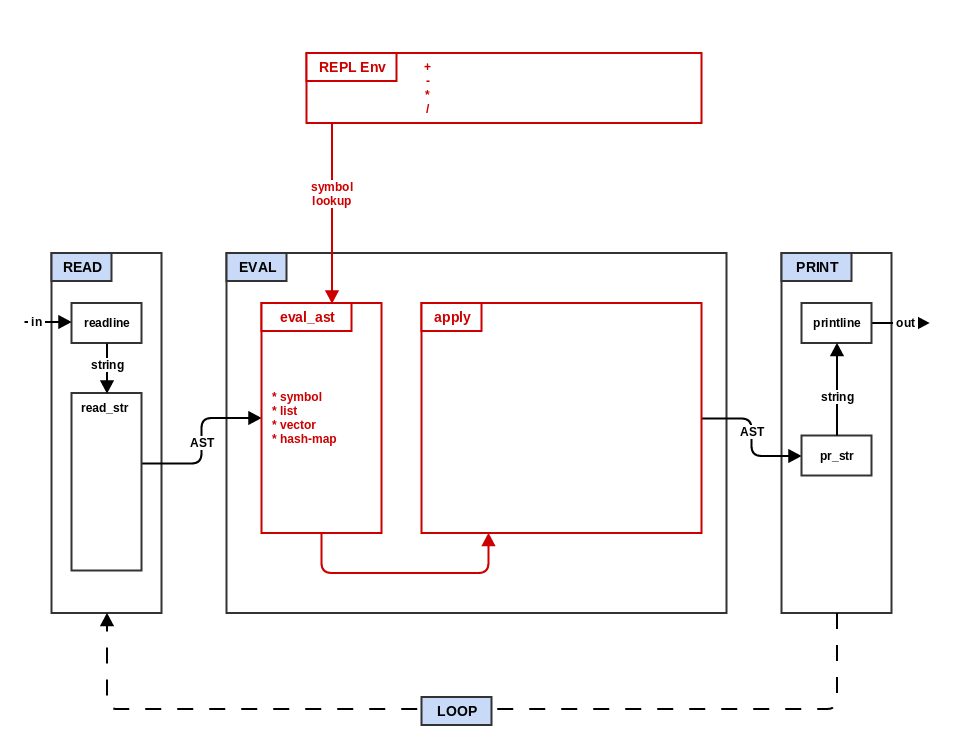
\includegraphics[width=.9\linewidth]{./images/step2_eval.png}
\end{frame}

\begin{frame}[fragile,label=sec-3-11]{Schritt 2}
 \begin{itemize}
\item \texttt{EVAL} (Tree Walker)
\item Definition von REPL-Environment mit \texttt{+}, \texttt{-}, \texttt{*}, \texttt{/}
\item Symbole im Environment nachschlagen
\item Skalar evaluiert zu seinem Wert
\item Liste wird als Funktionsaufruf (Apply-Phase) interpretiert:
\item Jedes Argument evaluieren, nachgeschlagene Funktion mit Argumenten
aufrufen
\item Sonderfall: Leere Liste
\item Resultat: Taschenrechner
\end{itemize}
\end{frame}

\begin{frame}[label=sec-3-12]{Schritt 3}
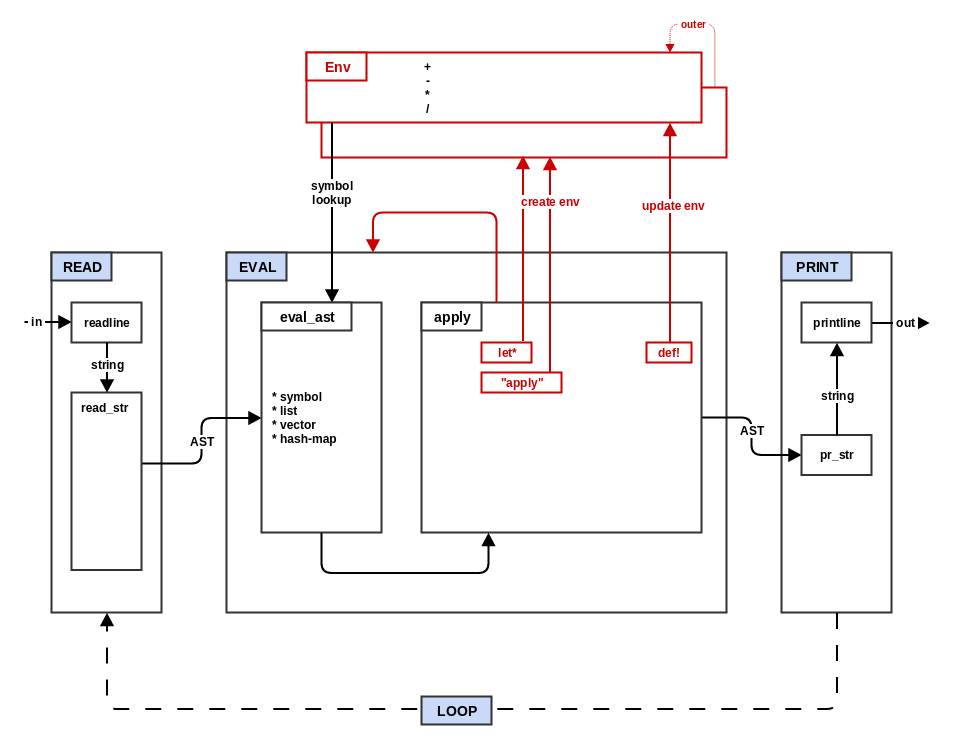
\includegraphics[width=.9\linewidth]{./images/step3_env.png}
\end{frame}

\begin{frame}[fragile,label=sec-3-13]{Schritt 3}
 \begin{itemize}
\item Environment: Outer Environment + Bindings
\item Binding: Name -> Wert
\item \texttt{let*}, \texttt{def!}: Spezielle Formen, besonders behandelt in \texttt{EVAL}
\item Normale Formen werden wie Funktionsaufrufe behandelt
\item \texttt{let*} erzeugt ein neues Environment mit gegebenen Bindings
\item \texttt{def!} mutiert Bindings in aktuellem Environment
\item Resultat: Taschenrechner mit Speicherfunktion
\end{itemize}
\end{frame}

\begin{frame}[label=sec-3-14]{Schritt 4}
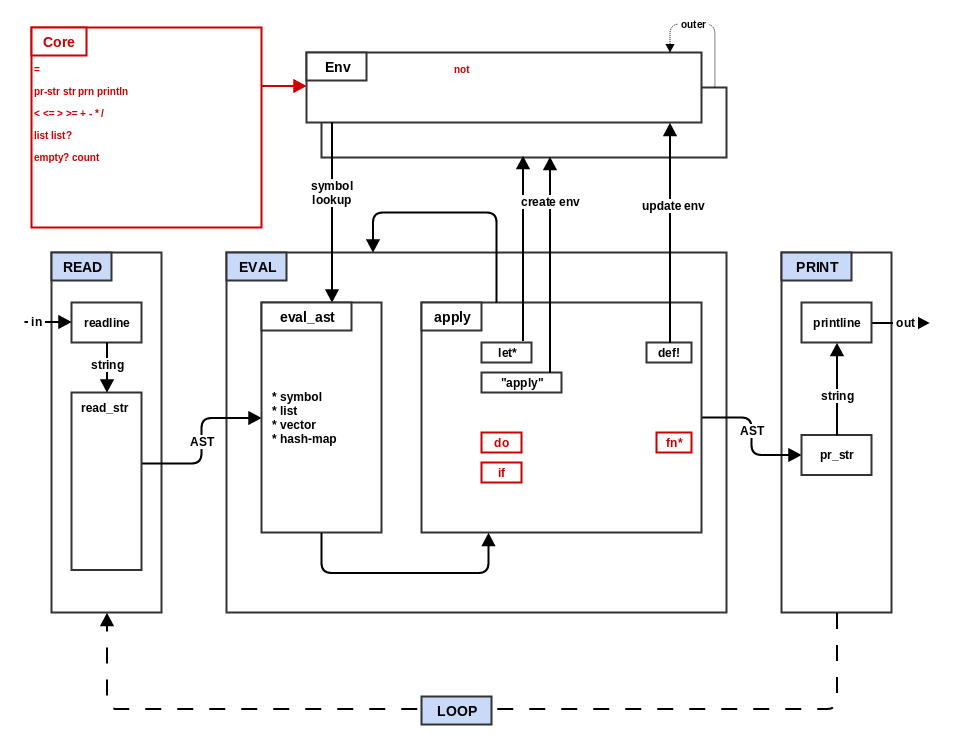
\includegraphics[width=.9\linewidth]{./images/step4_if_fn_do.png}
\end{frame}

\begin{frame}[fragile,label=sec-3-15]{Schritt 4}
 \begin{itemize}
\item \texttt{fn*} erzeugt benutzerdefinierte Funktion mit aktuellem Environment,
Argument-Liste und Body
\item Am einfachsten als Closure implementierbar die ein neues Environment
mit Argumenten erzeugt und Body damit evaluiert
\item Apply-Phase muss diesen Fall berücksichtigen
\item Alternativ \texttt{EVAL}-Sonderfall einführen
\item \texttt{if} und \texttt{do} müssen spezielle Formen sein, da besonderes Verhalten
\item Einführung einer Core-Datei mit weiteren Subrs
\item Resultat: Einfache Kontrollstrukturen
\end{itemize}
\end{frame}

\begin{frame}[label=sec-3-16]{Schritt 5}
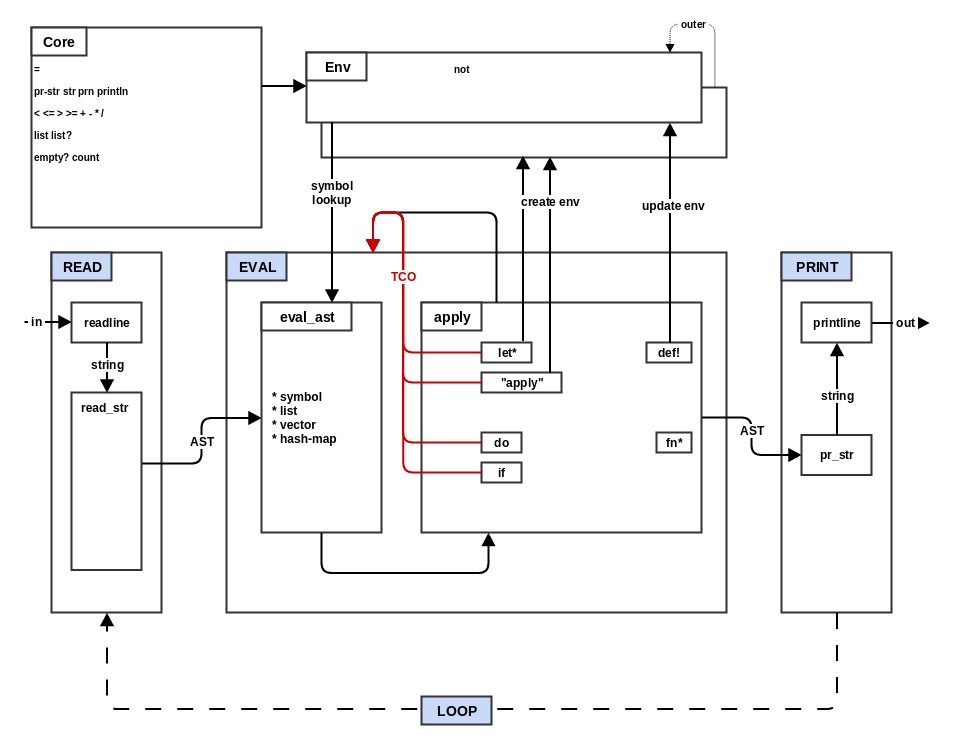
\includegraphics[width=.9\linewidth]{./images/step5_tco.png}
\end{frame}

\begin{frame}[fragile,label=sec-3-17]{Schritt 5}
 \begin{itemize}
\item TCO: Tail Call Optimization
\item Endrekursion verhält sich wie eine Schleife
\item Vermeiden neuer Stackframes, Rekursionslimit
\item Vielfältig implementierbar (GOTO, Trampolin, Cheney on the M.T.A.)
\item MAL verwendet eine Schleife in \texttt{EVAL} und \texttt{continue} für TCO-Fälle,
sonst \texttt{return}
\item Wichtig: Testen dass Code sich mit TCO identisch verhält
\item Resultat: Iteration durch Rekursion
\end{itemize}
\end{frame}

\begin{frame}[label=sec-3-18]{Schritt 6}
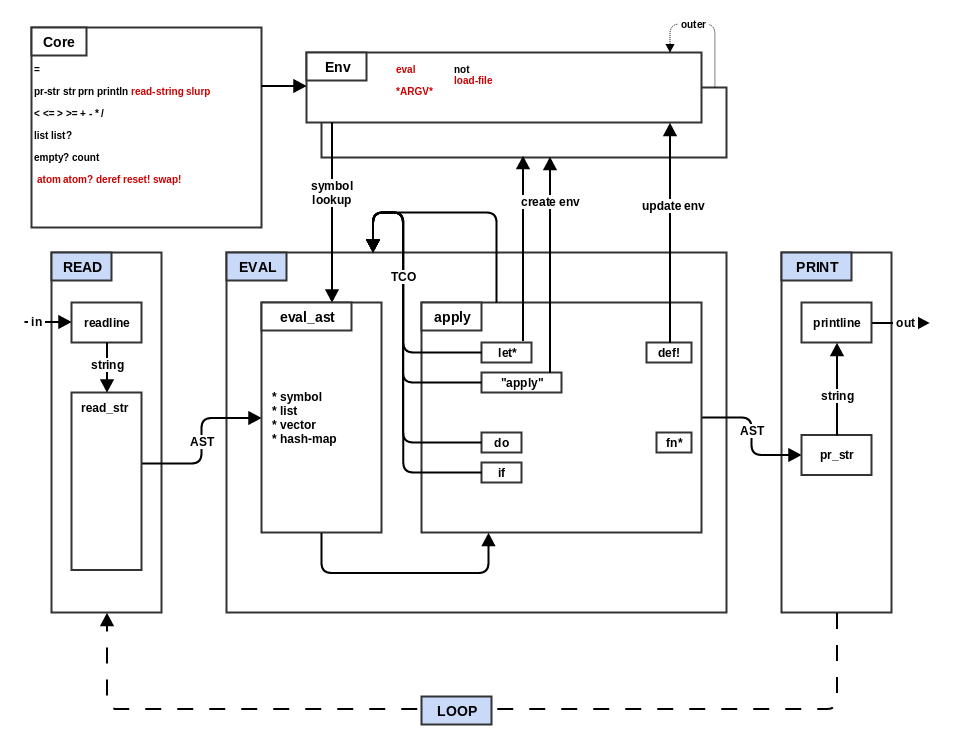
\includegraphics[width=.9\linewidth]{./images/step6_file.png}
\end{frame}

\begin{frame}[fragile,label=sec-3-19]{Schritt 6}
 \begin{itemize}
\item \texttt{eval} ist eine Closure die \texttt{EVAL} mit REPL-Environment ausführt
\item \texttt{read-string}
\item \texttt{slurp} für das Einlesen einer Datei
\item Implementierung von Atoms (mutierbarer State)
\item Wichtig: \texttt{apply} für \texttt{swap!} nötig
\item \texttt{load-file}: \texttt{(eval (read-string (str "(do" (slurp f) ")")))}
\item \texttt{*ARGV*} und Skriptmodus
\item Resultat: Interpreter kann Skripte ausführen
\end{itemize}
\end{frame}

\begin{frame}[label=sec-3-20]{Schritt 7}
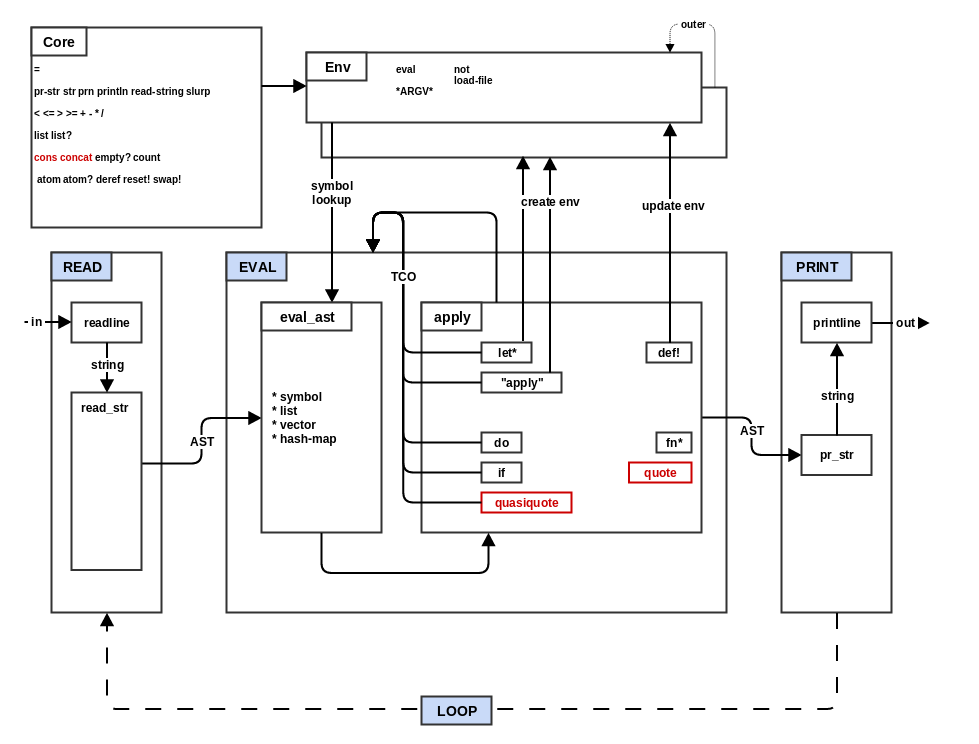
\includegraphics[width=.9\linewidth]{./images/step7_quote.png}
\end{frame}

\begin{frame}[fragile,label=sec-3-21]{Schritt 7}
 \begin{itemize}
\item Bisher nicht möglich etwas zum Symbol zu evaluieren
\item \texttt{quote} gibt das Argument unverändert zurück
\item \texttt{(quote foo)} -> \texttt{foo}, \texttt{(quote (1 2 3))} -> \texttt{(1 2 3)}
\item \texttt{quasiquote} erlaubt teilweises Evaluieren der Liste mit \texttt{unquote}
  und \texttt{splice-unquote}
\item \texttt{(let* [x '(2 3)] `(1 \textasciitilde{}x))} -> \texttt{(1 (2 3))}
\item \texttt{(let* [x '(2 3)] `(1 \textasciitilde{}@x))} -> \texttt{(1 2 3)}
\item Listenmanipulation in \texttt{EVAL}
\item Resultat: Vorbereitung auf Makros
\end{itemize}
\end{frame}

\begin{frame}[label=sec-3-22]{Schritt 8}
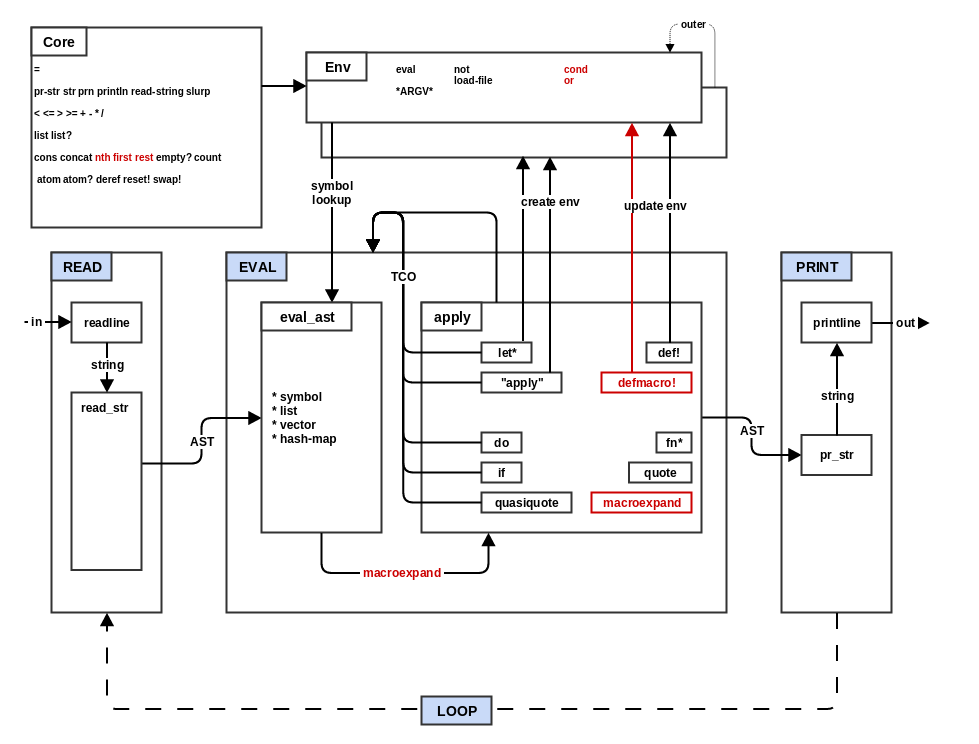
\includegraphics[width=.9\linewidth]{./images/step8_macros.png}
\end{frame}

\begin{frame}[fragile,label=sec-3-23]{Schritt 8}
 \begin{itemize}
\item Benutzerdefinierte spezielle Formen
\item Argumente werden nicht evaluiert
\item Makro-Aufruf wird durch Expansion ersetzt
\item \texttt{defmacro!} markiert ein Symbol als Makro
\item Expansion geschieht in \texttt{EVAL} als erster Schritt
\item \texttt{(defmacro! comment (fn* [\& body] nil))}
\item \texttt{(comment (/ 1 0))} -> \texttt{nil}
\item \texttt{macroexpand} für Debugging
\item Resultat: Makros
\end{itemize}
\end{frame}

\begin{frame}[label=sec-3-24]{Schritt 9}
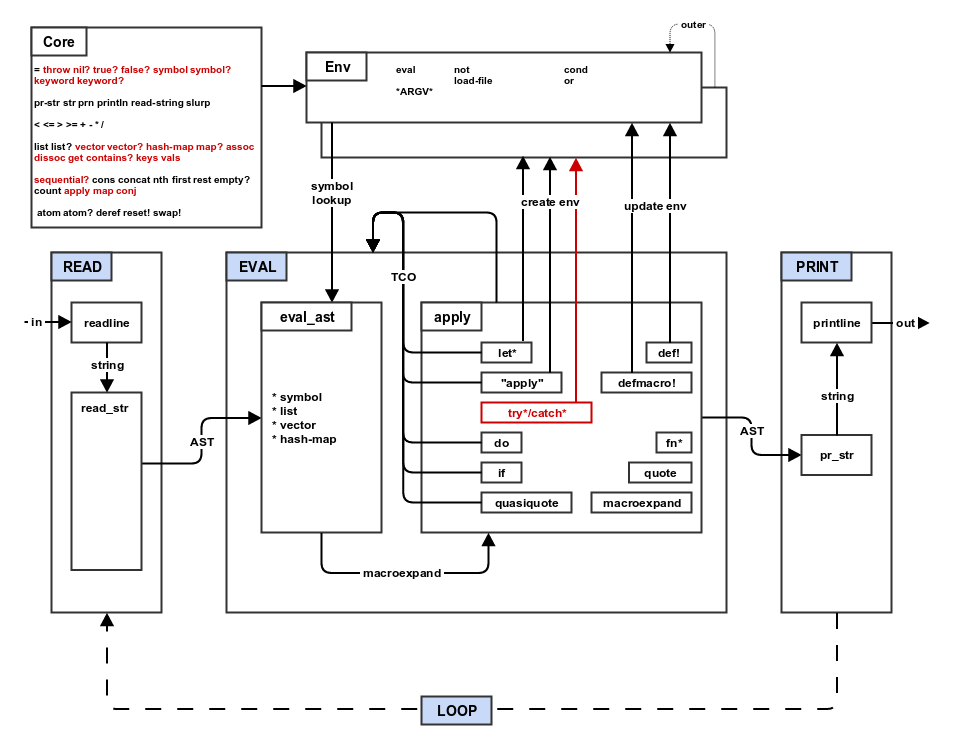
\includegraphics[width=.9\linewidth]{./images/step9_try.png}
\end{frame}

\begin{frame}[fragile,label=sec-3-25]{Schritt 9}
 \begin{itemize}
\item Exception Handling
\item \texttt{try*} fängt Exceptions, führt im Fehlerfall \texttt{catch*} aus
\item \texttt{throw*} wirft benutzerdefinierte Exception
\item Fortführung der Fehlerbehandlung aus \texttt{READ}
\item Falls Sprache Exceptions unterstützt, trivial, andernfalls mühselig
\item Taktiken: Globaler Fehlerstatus (\texttt{errno}), Fehlerobjekte
\item Implementierung der meisten fehlenden Subrs (inklusive \texttt{apply} und
\texttt{map})
\item Resultat: Brauchbare minimale Programmiersprache
\end{itemize}
\end{frame}

\begin{frame}[label=sec-3-26]{Schritt A}
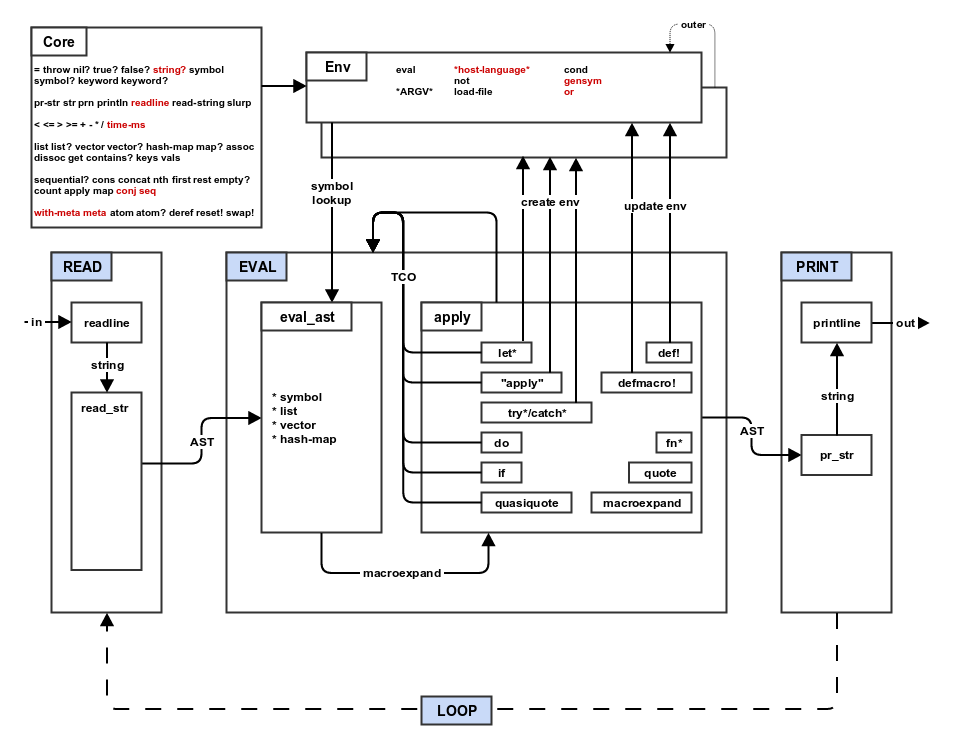
\includegraphics[width=.9\linewidth]{./images/stepA_mal.png}
\end{frame}

\begin{frame}[fragile,label=sec-3-27]{Schritt A}
 \begin{itemize}
\item Restliche Schritte für Self-Hosting
\item Metadaten-Support (\texttt{.clone}), \texttt{readline}, etc.
\item Ausführen der Implementierung in MAL im Skriptmodus
\item Debugging ist tricky
\item Finaler Schritt
\item Optional:
\begin{itemize}
\item Performance-Messung (\texttt{time-ms})
\item Interop (\texttt{.}, \texttt{<lang>-eval})
\end{itemize}
\end{itemize}
\end{frame}

\section{Weitere Schritte}
\label{sec-4}

\begin{frame}[label=sec-4-1]{Weitere Schritte}
\begin{itemize}
\item Einreichen einer neuen Implementierung
\item Diskussion und Verbesserung von MAL
\item Entwickeln einer eigenen Programmiersprache
\item PLT
\item Byte-Code Interpreter
\item Compiler
\item Scheme, Forth
\end{itemize}
\end{frame}

\begin{frame}[label=sec-4-2]{Lesematerial}
\begin{itemize}
\item \href{http://www.call-with-current-continuation.org/scheme-implementation-techniques.pdf}{Scheme Implementation Techniques}
\item Clojure-Sourcen
\item SICP
\item LiSP
\end{itemize}
\end{frame}

\begin{frame}[label=sec-4-3]{Fragen?}
\end{frame}
% Emacs 24.5.1 (Org mode 8.2.10)
\end{document}